\documentclass[oneside]{homework} %%Change `twoside' to `oneside' if you are printing only on the one side of each sheet.
\usepackage{setspace} 
\usepackage{algorithm} 
\usepackage{algorithmic}
\usepackage{multirow}
\usepackage{epsfig}
\renewcommand{\algorithmicrequire}{\textbf{Require:}}
\renewcommand{\algorithmicensure}{\textbf{Iteration:}}
\renewcommand{\algorithmiclastcon}{\textbf{Output:}}
\studname{Cheng Liu}
\collaborator{Introduction to algorithms\\}
\coursename{Analysis of algorithms I}
\hwNo{2}
\uni{cl3173}
\cuni{3rd edition}
\prNo{3}
\begin{document}
\maketitle
\newpage
\section*{Exercise 9.3-6}
Introduce Algorithm SELECT(A,i,n), the algorithm can pick up the  $n$th element in array A from index 0 to n.\\
And the worst case running time is $O(n)$. \\
\\ The pseduo-code is programming language independent ,then we just print each statistic.
\\ For those $n$ is not divisable by $k$, we the reminder as a addition to last group,no matter how large it will be.\\ 
\\ We set a variables to control the reminder named partition. To make the code more clear, we set the algorithm two steps.
  \begin{algorithm}[h]
  \caption{KthQuantilesStart}
  \label{algo:nlgkquantiles_start}
  \begin{algorithmic}[1]
	\REQUIRE A,k,n
	\ENSURE ~ ~\\ 
	  \STATE {$position = 0$}
	  \IF {$k==1$}
		\STATE {$PRINT \qquad n$}
		\STATE {$RETURN$}
	  \ELSIF {$k == 2$}
		\STATE {$position = SELECT(A,\lceil \frac{n}{2} \rceil,n)$ }
		\STATE {$PRINT\qquad position$ }
		\STATE {$RETURN$ }
	  \ELSE
	  \STATE {$partition = \lfloor \frac{n}{k} \rfloor $}
	  \STATE {$KthQuantilesProcedure(A,k,n,partition)$}
	  \ENDIF
	\LASTCON 	
  \end{algorithmic}
  \end{algorithm}
\\ It is easy to know that we find each kth order statistic in a binary way, thus we reduce the running time from $O(kn)$ to $O(n\log k)$.
\\ The recursion tree will be $\log k$ level and each level the cost will be about $O(n)$.
\\ The detail certification is omitted here, 
for $T(n) = T(\lceil n/2 \rceil ) + T(n-\lceil n/2 \rceil) + O(n) $ and stop when $T(k)$, a recursion tree can easily prove the correctness of the $O(n\log k)$running time.
\\ To prove the correctness of the algorithm, we notice that every SELECT function will return a certain K-th order statistic, when binary method is applied, the total times of call of SELECT funtion is $2^{\log k} = k$. Then all the K-th order statistic will be provided.
  \begin{algorithm}[h]
  \caption{KthQuantilesProcedure}
  \label{algo:nlgkquantiles_procedure}
  \begin{algorithmic}[1]
	\REQUIRE A,k,n,partition
	\ENSURE ~ ~\\ 
	  \STATE {$position = 0$}
	  \IF {$k==1$}
	  \STATE {$RETURN$}
	  \ELSIF {$k == 2$}
	  \STATE {$position = SELECT(A,\lceil \frac{n}{2} \rceil,n)$ }
	  \STATE {$PRINT\qquad position$ }
	  \STATE {$RETURN$ }
	  \ELSE
		\STATE {$position = SELECT(A, \lceil \frac{k}{2} \rceil partition,n)$ }
		\STATE {$L = \left\{x \in A, x \leq position\right\}$}
		\STATE {$H = \left\{x \in A, x > position\right\}$}
		\STATE {$KthQuantilesProcedure(L,\lceil \frac{k}{2} \rceil,\lceil \frac{k}{2} \rceil partition,partition)$}
		\STATE {$PRINT\qquad position$ }
		\STATE {$KthQuantilesProcedure(H,\lceil \frac{k}{2} \rceil,n-\lceil \frac{k}{2} \rceil partition,partition)$}
	  \ENDIF
	\LASTCON 	
  \end{algorithmic}
  \end{algorithm}

\section*{Exercise 9.3-8}
{\bfseries 
  Notice: since the total number of elements in the two arraies is even, then we take the mean of the median two numbers as the median of these two arraies.
}
  \begin{algorithm}[h]
  \caption{FindMedian}
  \label{algo:lgnmedian}
  \begin{algorithmic}[1]
	\REQUIRE X,xstart=0,xend=n,Y,ystart=0,yend=n
	\ENSURE ~ ~\\ 
	  \IF {$xstart = = xend$}
	  \STATE {$median = \frac{X[xstart]+Y[ystart]}{2}$}
	  \ELSIF {$X[\frac{xstart+xend}{2}] = = Y[\frac{ystart+yend}{2}]$}
	  \STATE {$median = X[\frac{xstart+xend}{2}]$ }
	  \ELSIF {$X[\frac{xstart+xend}{2}] \leq Y[\frac{ystart+yend}{2}]$}
	  \STATE {$median = FindMedian(X,\frac{xstart+xend}{2},xend,Y,ystart,\frac{ystart+yend}{2})$}
	  \ELSE
	  \STATE {$median = FindMedian(X,xstart,\frac{xstart+xend}{2},Y,\frac{ystart+yend}{2},yend)$}
	  \ENDIF
	\LASTCON $median$	
  \end{algorithmic}
  \end{algorithm}
\\In every recursion, the size of the two arraies is cutted by half, the maximum layer of recursion is $\lg 2n $, and in each recursion, the cost is just a constant $c$, then the total running time of the algorithm is just $O(\lg n)$.
\begin{figure}[!h]
  \centerline{
	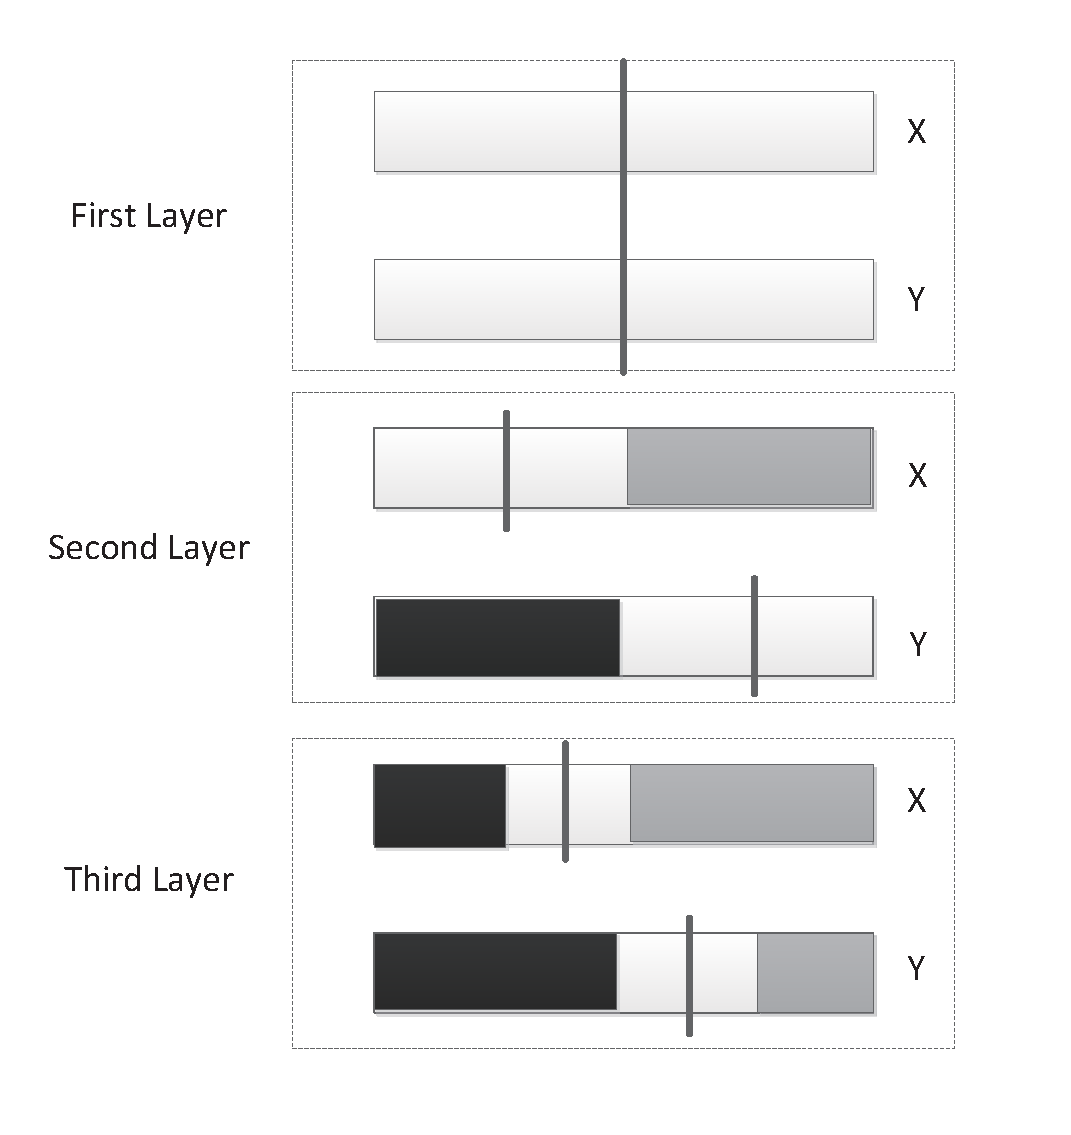
\epsfig{file=./hw2_3_1.eps, scale=0.4}
}
  \caption{Illustration of the Median Find Algorithm}
  \label{fig:illalgomedian}
\end{figure}
\\We illustrate the principle of the algorithm in Figure \ref{fig:illalgomedian}. \\This figure shows first 3 recursions of the algorithm, and the black vertical line indicates position to execute the comparison,denoting with lower index mid. The light shadow shows those numbers that have been determined to be larger than the median,and the heavy shadow shows those smaller numbers.
\\In the first recursion, we assume that the $X_{mid} > Y_{mid}$, then we know that median won't exsit in shadow area. If it is, for example, the median is in light shadow(indicating in layer 2), it will be larger than more than half of the X array elements and it will be also larger than half of the Y array elements, the total of these two part will exceeds $n$. \\
So it cannot be the median.\\ Similarly,it won't be heavy shadow area.\\So the median must be in the un-shadowed area.\\
Then we discard these two shadow parts and go into next section as it shown in the second layer. \\
This time, we can transfer the original problem to find the median of the remaining two sorted arraies with length of $\frac{n}{2}$.\\
The procedure of the second layer is just the same as the first layer. With recursion going deeper, the remaining part of the arries will be smaller and smaller to reach only two elements, and we can similarly prove that the median is always staying with the recursion, then we take the mean of them as the median.\\ And it will be probable that the two mid elements are equal,then they are both the median. 
\end{document}
